\documentclass{article}

\usepackage{graphicx}
\usepackage{hyperref}
\usepackage{bm}
\usepackage{float}
\restylefloat{table}

\usepackage{listings}
\usepackage{color}
\usepackage{amsmath}

\usepackage[margin=1.25in]{geometry}

\definecolor{dkgreen}{rgb}{0,0.6,0}
\definecolor{gray}{rgb}{0.5,0.5,0.5}
\definecolor{mauve}{rgb}{0.86,0.27,0.22}

\lstset{frame=tb,
  language=python,
  aboveskip=3mm,
  belowskip=3mm,
  showstringspaces=false,
  columns=flexible,
  basicstyle={\small\ttfamily},
  numbers=left,
  stepnumber=1,
  numberstyle=\tiny\color{gray},
  keywordstyle=\color{blue},
  commentstyle=\color{dkgreen},
  stringstyle=\color{mauve},
  breaklines=true,
  breakatwhitespace=true,
  tabsize=3
}

\title{CS5200: Prelim Exam \#2} % Title of the assignment

\author{Matthew Whitesides\\ \texttt{mbwxd4@umsystem.edu}} % Author name and email address

\date{\today} % University, school and/or department name(s) and a date

%----------------------------------------------------------------------------------------

\begin{document}

  \maketitle % Print the title

  \textit{I, Matthew Whitesides, certify that all the material in this PDF file is my original work, that I did not discuss these questions with anyone other than my instructor, and that I did not copy work from anyone for this examination.}
 
  \begin{enumerate}
    \item \textbf{Probability}.
    
    First let's setup our sample space. Given that it dosen't really matter what disk we change lets say disk one stays the same and we place disk two on top and rotate it.

    Disk two will have 128 possible differnt positions it can be placed on top of disk one. Therefore:
    
    \[S=\{1,2,...,128\}\]

    Now let's define for each $i$ in the sammple space $S$, we have a $j$ meaning if $i = 1$ that sector 1 of the second disk is placed ontop of sector $j$ of the first disk.

    Next let's define a random variable $S\rightarrow R$ given by Matches(j) = the number of matches when disk two's slice 1 is over disk one's slick $j$.

    Now since we have a sample space of 128 we'll need to calculate the matches for each sector using indicator variables.\\

    Let's define $M_i:S\rightarrow R$ meaning matches given sample space i given by:

    $M_i(j) = 1$ If sector $i$ of disk two has a match over disk one's sector $j$.

    $M_i(j) = 0$ If no match.

    Therefore the total matches would be the sum of each indicator variable:

    \[\sum_{i=1}^{128}E(M_i)\]

    Now we just need to calcualte the chance there's a match or no match for any given sector.

    Our possibile probability for each sector are (position one being color of disk one and two being two) with RR, WW being matches and RW, WR being not:

    \[\{RR, RW, WR, WW\} = \{\frac{1}{4} \frac{1}{2}, \frac{1}{4} \frac{1}{2}, \frac{3}{4} \frac{1}{2}, \frac{3}{4} \frac{1}{2}, \}\]

    And doing this you can easily see that the odds of getting a match are the same as not getting a mtach with it being more likely to get a WW match. Therefore:

    \[E(M_i) = 1(\frac{1}{2}) + 0(\frac{1}{2}) = \frac{1}{2}\]

    And thus our expected matches, \bm{$E(Matches) = 128 * \frac{1}{2} = 64$} meaning we can always expect to be able to place disk two ontop disk one to get at least 64 matches.

    \item \textbf{Induction}.
    
    Proof.
    
    \begin{itemize}
      \item The Problem:
      \begin{itemize}
        \item Let $P(C)$ be for any complete 4-tree the number of leaves can be calculated by $L = 3C + 1$.
        \item A complete tree is defined as each node has 4 children except the highest level nodes when are called leaves which have 0. 
        \item Let L = \# of leaves
        \item and C = \# of complete nodes.
        \item The domain is all natural number values of $C \geq 0$. As a negitive or partial number of nodes would not make sense.
      \end{itemize}
      \item The Inductive Stopping Values:
      \begin{itemize}
        \item Base case: C = 0.
        \begin{itemize}
          \item $L = 3(0) + 1 = 1$. 
          \item True as you have 0 "complete" nodes and one "leaf" node with 0 children.          
        \end{itemize}
        \item Base case: C = 1.
        \begin{itemize}
          \item $L = 3(1) + 1 = 4$. 
          \item True as you have one "comeplete" node with 4 children leaves.          
        \end{itemize}
        \item Next step: C = 2.
        \begin{itemize}
          \item $L = 3(2) + 1 = 7$. 
          \item True as you have the root node wtih one non leaf child leaving 3 leaves and that child having 4 leaves.          
        \end{itemize}
        \item Next step: C = 3.
        \begin{itemize}
          \item $L = 3(3) + 1 = 10$. 
          \item True as you'd have a tree like the following (with the green being the leaf nodes).\\
          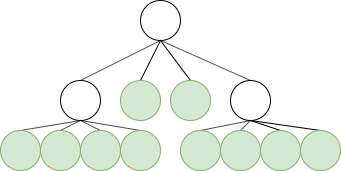
\includegraphics[scale=0.3]{2a.png}
        \end{itemize}        
      \end{itemize}
      \item For any $C \geq 0$ if $P(C)$ is true then $P(C + 1)$ must also be true.
      \begin{itemize}
        \item Assume that hypothesis for some value of $P(C)$ is true then we must show that $P(C + 1)$ is true.
        \item We can show this using the induction hpyothesis with an equation like so.
        \[(3C + 1) + 3(1) = 3(C + 1) + 1\]
        \item which using simple algebra is true.
      \end{itemize}
      \item Since steps 0 - 3 have been verified and we have shown that for every value if $P(C)$ is true then $P(C + 1)$ is true, therefore $L = 3C + 1$ for all natural number values of C.
    \end{itemize}

    \item \textbf{Proof by Induction}.
    \begin{enumerate}
      \item 
      \begin{lstlisting}
  def f(n):
    if n <= 0:
        return 4
    elif n <= 1:
        return 32
    else:
        return 8*f(n - 1) - 16*f(n - 2)

  print("f(0) = ", f(0))
  print("f(1) = ", f(1))
  print("f(2) = ", f(2))
  print("f(3) = ", f(3))

  #Output:
  f(0) =  4
  f(1) =  32
  f(2) =  192
  f(3) =  1024
      \end{lstlisting}

      Like the hint says lets look $4^n$. 

      \begin{lstlisting}
  print("4**0 = ", 4**0, ", diff = ", f(0) - 4**0, ", f(n)/4^n = ", f(0) / 4**0)
  print("4**1 = ", 4**1, ", diff = ", f(1) - 4**1, ", f(n)/4^n = ", f(1) / 4**1)
  print("4**2 = ", 4**2, ", diff = ", f(2) - 4**2, ", f(n)/4^n = ", f(2) / 4**2)
  print("4**3 = ", 4**3, ", diff = ", f(3) - 4**3, ", f(n)/4^n = ", f(3) / 4**3)
  print("4**4 = ", 4**4, ", diff = ", f(4) - 4**4, ", f(n)/4^n = ", f(4) / 4**4)
  print("4**5 = ", 4**5, ", diff = ", f(5) - 4**5, ", f(n)/4^n = ", f(5) / 4**5)

  #Output:
  4**0 =  1 , diff =  3 , f(n)/4^n =  4.0
  4**1 =  4 , diff =  28 , f(n)/4^n =  8.0
  4**2 =  16 , diff =  176 , f(n)/4^n =  12.0
  4**3 =  64 , diff =  960 , f(n)/4^n =  16.0
  4**4 =  256 , diff =  4864 , f(n)/4^n =  20.0
  4**5 =  1024 , diff =  23552 , f(n)/4^n =  24.0
      \end{lstlisting}

      Looking at the difference you can pretty easily see the difference between $4^n$ and $f(n)$ plus $4^n$ gives us $f(n + 1)$.
      
      Also if we look at $f(n) / 4^n$ we can see that $f(n) / 4^n = 4(n + 1)$.\\

      Therefore we can decude that \bm{$f(n) = 4^n(4(n + 1))$}.
      
    \end{enumerate}
  \end{enumerate}  
\end{document}
